\section{Technical Approach}
\label{sec:method}
\paragraph{Data Preprocessing}
\paragraph{Architecture Implementation and Validation}
The overall architecture of our model is illustrated in Figure 1. In this design, the base model utilized for patch-level prediction is the ArtNet model.\\
During inference, the input image is first divided into five patches—top left, top right, bottom left, bottom right, and center. Each patch is then independently processed by the baseline model to produce a probability distribution over the five artistic style classes. These five probability vectors are subsequently concatenated and fed into a shallow neural network, which produces the final style classification.\\
The primary objective of this stage is to validate that integrating a shallow decision-making network into the prediction pipeline leads to higher classification accuracy compared to directly using the baseline model for whole-image prediction.
\begin{figure}[h]
    
    \centering
    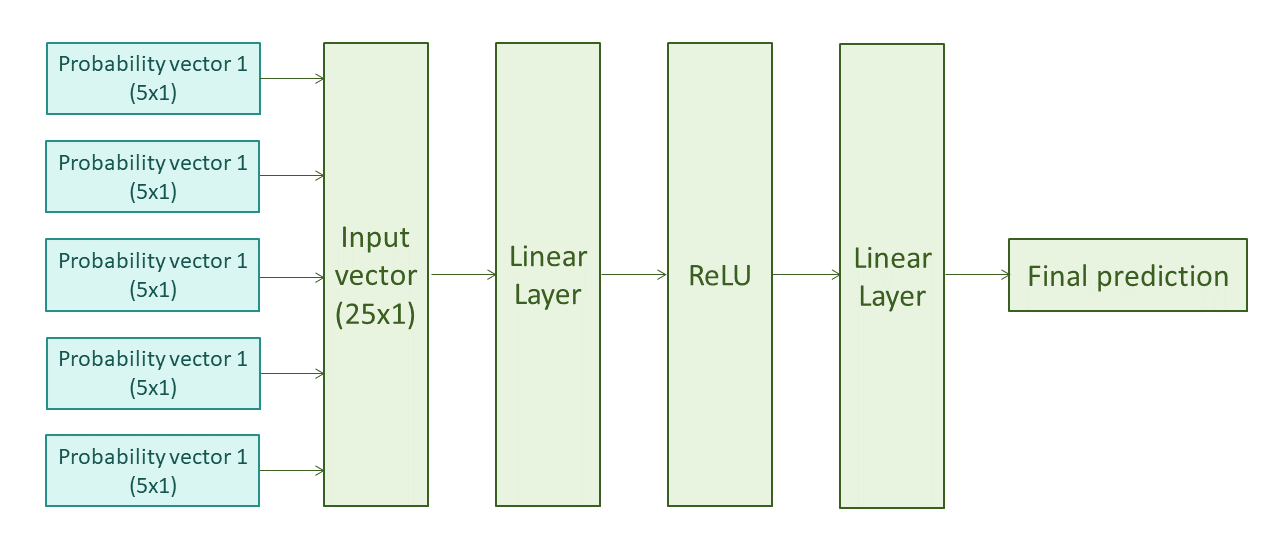
\includegraphics[width=.45\textwidth]{shallownn.png}
    \caption{Shallow NN architecture}
    \label{fig:main_pipeline}
\end{figure}

The architecture of the shallow neural network, consisting of a single hidden layer, is shown above.
By utilizing the prepared training data—comprising five probability vectors as inputs and the corresponding ground truth labels as outputs—the shallow network can be trained to learn the mapping parameters. Once trained, the shallow network is directly employed during inference to generate the final style prediction.
\paragraph{Adaptive Refinement and Optimization}
\begin{itemize} \item \textbf{Selection of the Fifth Patch:}
We propose two strategies for selecting the fifth patch: \begin{itemize} \item \textit{Global Context Patch:} The original image is resized to match the patch size and directly used as the fifth patch. This approach aims to incorporate global contextual information, which is expected to enhance classification accuracy. \item \textit{Semantic-Driven Patch:} A patch containing the most salient semantic content is detected and selected as the fifth patch. This method focuses on capturing the most informative region of the image to assist the decision-making network in improving prediction performance. \end{itemize} \item \textbf{Architectural Variations:}
We also explore more advanced hierarchical architectures for patch selection and decision aggregation. In particular, we investigate the use of architectures such as the Swin Transformer~\cite{9718928}, and analyze their impact on the overall classification accuracy. \end{itemize}